% presentation
\documentclass{beamer}

% \usetheme{Boadilla}
\usetheme{Warsaw}

% rus lang
\usepackage[main=russian,english]{babel}

% insert images
\usepackage{wrapfig}

% for svg images
% !TeX TXS-program:compile = txs:///pdflatex/[--shell-escape]
\usepackage{svg}
	
\title{Лекция 1. Введение}
\subtitle{Основы интеллектуального анализа данных}
\author{Полузёров Т. Д.}
\institute{БГУ ФПМИ}
\date{}


\begin{document}
	
	
	\begin{frame}
		\titlepage
	\end{frame}
	
	
	\begin{frame}
		\frametitle{Структура лекции}
		\tableofcontents
	\end{frame}


	\section{О чем предмет}
	
	
	\begin{frame}
		\frametitle{Цели анализа данных}
		\textbf{Data mining} - процесс извлечения знаний из различных источников данных (базы данных, текст, картинки). Полученные знания должны быть достоверными, полезными, интерпретируемыми.
		
		\vspace{5pt}
				
		\textbf{Моделирование} - процесс построения модели, хорошо описывающей закономерности, которые порождают данные.
		
		\vspace{5pt}		
		
		Подходы к построению моделей:
		\begin{itemize}
			\item статистический
			\item на основе машинного обучения
			\item вычислительный
		\end{itemize}
		
	\end{frame}
	
	
	\begin{frame}
		\frametitle{Типы задач}
		Основные две группы задач: 
		
		\begin{itemize}
			\item Обучение с учителем:
			\begin{itemize}
				\item Регрессия - прогноз численного значения 
				\item Классификация - определения класса объекта
				\item Ранжирование - упорядочивание объектов
			\end{itemize}
		
			\item Обучение без учителя:
			\begin{itemize}
				\item Кластеризация - выделение семейств, групп в данных
				\item Поиск ассоциативных правил - поиск зависимых событий
				\item Понижение размерности - сжатие данных при разумной 
				потере информации
			\end{itemize}
		\end{itemize}
	\end{frame}

	
	\begin{frame}
		\frametitle{Этапы решения задач}
		Классическая схема решения задачи состоит из этапов:
		\begin{enumerate}
			\item Определение задачи которую нужно решить
			\item Сбор и подготовка данных
			\item Определение используемых инструментов, моделей
			\item \textbf{Построение модели}
			\item \textbf{Первичная оценка качества модели (offline evaluation)}
			\item Внедрение или доработка модели
			\item Оценка результатов работы в продакшене (online evaluation)
			
		\end{enumerate}
	\end{frame}
	
	
	
	
	\section{Основные обозначения}
	
	
	\begin{frame}
		\frametitle{Постановка задачи. Обучение с учителем}
		
		$\mathbb{X}$ - множество объектов
		
		$\mathbb{Y}$ - множество ответов
		
		$y^{*}: \mathbb{X} \to \mathbb{Y}$ -неизвестная зависимость (target function)
		
		\vspace{15pt}
		
		\textbf{Дано}:
		
		$X = \{x_1, ..., x_\ell\} \subset \mathbb{X}$ - обучающая выборка (samples)
		
		$Y = \{y_1, ..., y_{\ell}\} = \{y^{*}(x_i), i = 1...\ell \} \subset \mathbb{Y}$ - известные ответы (targets)
		
		\vspace{5pt}
		
		\textbf{Необходимо}:
		
		Найти алгоритм (решающую функцию, модель) $a: \mathbb{X} \to \mathbb{Y}$ приближающую $y^{*}$ \textbf{на всём} множестве $\mathbb{X}$		
	\end{frame}


	\begin{frame}
		\frametitle{Признаковое описание объектов}
		
		Отображения $f_j: \mathbb{X} \to D_j, j=1, ..., n$ - признаки объекта (features), измерение некоторох характеристик объекта
		
		
	
		Вектор $(f_1(x), ..., f_n(x))$ - признаковое описание объекта $x$.
		
		\vspace{5pt}
		
		Матрица "объекты-признаки":
		
		 $$
		 F = (f(x_{ij}))_{\ell \times n} = 
		 \begin{pmatrix}
		 	f_{1}(x_1) & ... & f_{n}(x_1) \\
		 	... & ... & ... \\
		 	f_{1}(x_{\ell}) & ... & f_{n}(x_{\ell}) \\		 	
		 \end{pmatrix}
		 $$
		 
		 Далее будем отождествлять признаковое описание объекта с самим объектом:
		 
		 $x := (f_1(x), ..., f_n(x))$
		 , т.е. $X := F$
	\end{frame}
		
	
	\begin{frame}
		\frametitle{Типы признаков}
		Основные типы признаков:
		\begin{itemize}
			\item $D_j = \{0, 1\}$ - \textbf{бинарный} признак $f_j$
			\item $|D_j| < \infty$ и определена только операция сравнения на равенство - \textbf{категориальный} признак$f_j$
			\item $|D_j| < \infty$ $f_j$ и определены операции сравнения больше, меньше, равенство - \textbf{порядковый }(ранговый) признак $f_j$
			\item $D_j \subseteq \mathbb{R}$ - \textbf{количественный} признак $f_j$
		\end{itemize}
	
		\vspace{5pt}
		
		Примеры:
		\begin{itemize}
			\item Цвет - категориальный признак, нельзя сказать "Красный" $>$ "Синий"
			\item Офицерские звания - пример порядкового признака, можно ортировать категории
			\item Время/дата - может проявлять свойства непрерывных, категориальных, циклических типов
		\end{itemize}
	\end{frame}
	
	
	\begin{frame}
		\frametitle{Форма множества ответов - определяет тип задачи}
		
		Задача классификации:
		\begin{itemize}
			\item $\mathbb{Y} = \{0, 1\}$ - бинарная классификация
			\item $\mathbb{Y} = \{1, ... M\}$ - на $M$ непересекающихся классов (multiclass)
			\item $\mathbb{Y} = \{0, 1\}^{M}$ - на $M$ классов, которые могут пересекаться (multilabel)
		\end{itemize}
		
		\vspace{5pt}
		
		Восстановления регрессии:
		\begin{itemize}
			\item $\mathbb{Y} = \mathbb{R}$ 
			\item $\mathbb{Y} = \mathbb{R}^{m}$
		\end{itemize}
	
		\vspace{5pt}
		
		% \ после кавычек - для их сохранения, можно {} вместо \
		В задачах "обучения без учителя"\ - множество $\mathbb{Y}$ не определено
	\end{frame}


	\begin{frame}
		\frametitle{Модель - как семейство параметризованных функций}
		
		\textbf{Модель} - параметрическое семейство функций
		$$
		\mathbb{A} = \{a(x, \theta) | \theta \in \Theta\}
		$$
		
		где $a: \mathbb{X} \times \Theta \to \mathbb{Y}$ - фиксированная функция,
		$\Theta$ - множество допустимых значений $\theta$
		
		\vspace{15pt}
		
		Пример:
		
		\begin{itemize}
			\item $\{a(x) = \sum_{j=1}^{n} \omega_j x_j\ | \omega_j \in \mathbb{R}\}$ - семейство линейных моделей для задачи регрессии, $\mathbb{Y} = \mathbb{R}$
			
			\item $\{a(x) = [(\sum_{j=1}^{n} \omega_j x_j) > 0] | \omega_j \in \mathbb{R}\}$ - семейство линейных моделей для бинарной классификации, $\mathbb{Y} = \{0, 1\}$
		\end{itemize}
	\end{frame}


	\begin{frame}
		\frametitle{Метод обучения}
		
		\textbf{Метод обучения} (learning algorithm) - это отображение вида
		$$
		\mu : (\mathbb{X} \times \mathbb{Y}) \to \mathbb{A}
		$$
		
		которое произвольной конечной выборке $(X \times Y) = \{(x_i, y_i\}_{i=1}^{\ell}$ ставит в соответствие 
		некоторый алгоритм $a \in \mathbb{A}$
		
		\vspace{15pt}
		
		\textbf{Обучить модель} (fit) - значит с помощью метода обучения $\mu$ определить конкретные значения параметров для модели из выбранного семейства.
	\end{frame}


	\begin{frame}
		\frametitle{Функционалы качества}
		
		$\mathcal{L}(a, x)$ - \textbf{функция потерь} (loss function)  - неотрицательная функция пропорциональная величине ошибки алгоритма $a \in \mathbb{A}$ на объекте $x \in \mathbb{X}$, если верный ответ есть $y \in \mathbb{Y}$
		
		\vspace{5pt}
		
		Функции потерь для задач классификации:
		\begin{itemize}
			\item $\mathcal{L}(a, x) = [a(x) \not= y]$ - индикатор ошибки
		\end{itemize}
		
		Функции потерь для задач регрессии:
		\begin{itemize}
			\item $\mathcal{L}(a, x) = |a(x) - y|$ - абслолютное значение ошибки
			\item $\mathcal{L}(a, x) = (a(x) - y)^2$ - квадрат ошибки
		\end{itemize}
		
		\vspace{5pt}
		
		\textbf{Эмпирический риск} - функционал качества алгоритма $a$ на конечной выборке $X \subset \mathbb{X}$
		$$
		Q(a, X) = \frac{1}{\ell} \sum_{i=1}^{\ell} \mathcal{L}(a, x_i)
		$$
	\end{frame}		
		
		
	\begin{frame}
		\frametitle{Основной метод обучения}
		Метод \textbf{минимизации эмпирического риска}:
		$$
		\mu(X) = arg \min_{a \in A} Q(a, X)
		$$
		
		Пример: метод наименьших квадратов, $Y = \mathbb{R}, \mathcal{L}$ - квадратична
		$$
		\mu(X) = arg \min_{a \in A} \sum_{i=1}^{\ell} (a(x_i, \theta) - y_i)^{2}
		$$
		
		\vspace{5pt}
		
		Два этапа модели:
		\begin{itemize}
			\item Этап обучения (fit): по имеющейся выборке $X$ с помощью метода обучения $\mu$ построить $a$.
		
			\item Этап применения обученной модели (predict): $\hat{y}_i = a(x_i^{'})$
		\end{itemize}
	\end{frame}
		
	\begin{frame}
		\frametitle{Обобщающая способность}
		Если минимум функционала $Q(a, X)$ достигается на алгоритме $a$, то это еще не гарантирует, что $a$ будет хорошо приближать целевую зависимость на произвольной контрольной выборке $X^{'} \in \mathbb{X}$
		
		\vspace{15pt}
		
		\textbf{Обобщающая способность} метода $\mu$ характеризуется величиной $Q(\mu(X), X^{'})$, где $X$ и $X^{'}$ получены из одного и того же неизвестного распределения $\mathbb{X}$
		
		\vspace{15pt}
		
		Крайние ситуации при обучении:
		\begin{itemize}		
			\item \textbf{Недообучение} - ситуация, когда качество плохое и на $X$, и на $X^{'}$
			\item \textbf{Переобучение} - качество на $X$ хорошее, но на $X^{'}$ существенно хуже
		\end{itemize}
		
	\end{frame}

	
	\begin{frame}
		\frametitle{Пример недо- и переобучения}
		
		% svg package
		%\includesvg[width=\textwidth]{img/overtraining}
		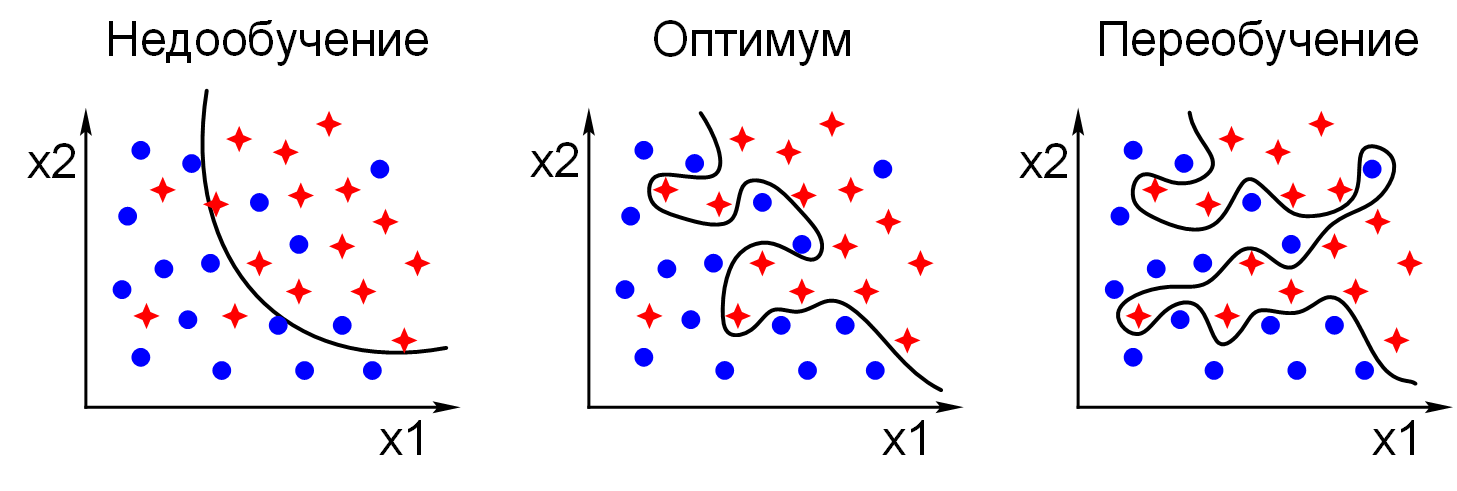
\includegraphics[width=\textwidth]{img/overfit1.png}
		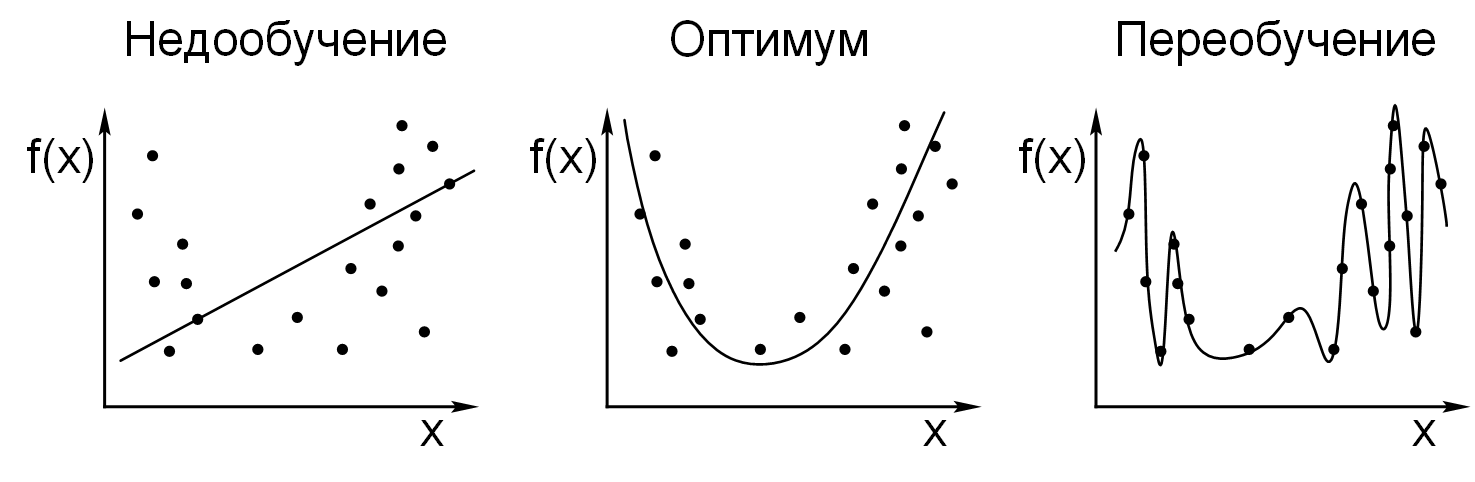
\includegraphics[width=\textwidth]{img/overfit2.png}
	\end{frame}


	\begin{frame}
		\frametitle{Переобучение - проблема обобщающей способности}

			\textbf{Из-за чего возникает переобучение?}
			Избыточная сложность пространства параметров $\Theta$ позволяет черезмерно точно подстроиться под обучающую выборку. Переобучение есть всегда, когда оптимизация идет по конечной выборке
			
			\vspace{15pt}
			
			\textbf{Избавиться нельзя. Как минимизировать?}
			\begin{itemize}
				\item Использовать класс более "простых" моделей
				\item Накладывать ограничение на параметры модели - регуляризация
				\item Увеличить обучающую выборку
			\end{itemize}
	\end{frame}


	\begin{frame}
		\frametitle{Эмпирические оценки обобщающей способности}
		\begin{itemize}
			\item Отложенная выборка (hold-out), $X = X_{train} \sqcup X_{test}$
			$$
			HO(\mu, X_{train}, X_{test}) = Q(\mu(X_{train}), X_{test}) \to min
			$$
			
			\item Скользящий контроль (leave-one-out):
			$$
			LOO(\mu, X) = \frac{1}{L} \sum_{i=1}^{L} Q(\mu(X \setminus \{x_i\}), x_i) \to min
			$$
			
			\item Кросс-проверка (cross-validation), 
			$X = X_1 \sqcup X_2 \sqcup ... \sqcup X_k$
			%$L = \ell + k, X^{L} = X_{n}^{\ell} \sqcup X_{n}^{k}$:
			$$
			CV(\mu, X^{L}) = \frac{1}{k} \sum_{i=1}^{k} Q(\mu(X \setminus X_{k}), X_{k}) \to min
			$$
		\end{itemize}
	\end{frame}
	
	
	\begin{frame}
		\frametitle{Кросс-валидация}
		
		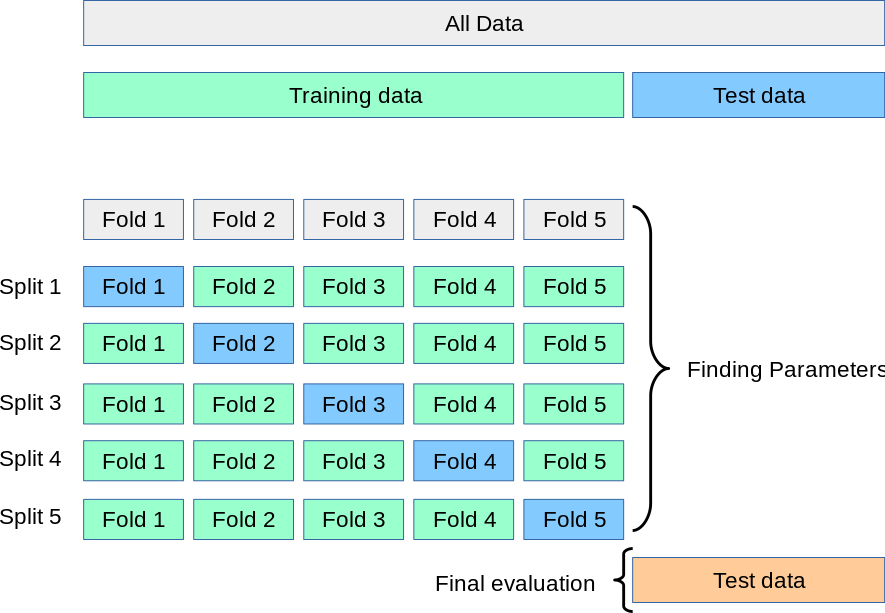
\includegraphics[width=0.9\textwidth]{img/cv.png}
	\end{frame}
	
	\section{Примеры реальных задач}
	
	
	\begin{frame}
		\frametitle{Кредитный скоринг}
		Объекты - заявки клиентов на кредит
		
		Цель - одобрить или отклонить заявку
		
		\vspace{5pt}
		
		Признаки:
		\begin{itemize}
			\item Бинарные: пол, наличие авто, имеет ли действующие кредиты
			\item Непрерывные: зарплата, сумма кредита
			\item Порядковые: образование, должность
			\item Категориальные: тип кредита, семейный статус
		\end{itemize}
	
		Особенности задачи:
		\begin{itemize}
			\item Дисбаланс классов: очень мало дефолтных
			\item Требование оценки вероятности дефолта
			\item Интерпретируемость модели
		\end{itemize}
	\end{frame}
	
	
	\begin{frame}
		\frametitle{Отток клиентов}
		Объекты - абонент в определенный момент времени
		
		Цель - распознавать риск ухода клиента
		
		\vspace{5pt}
		
		Признаки:
		\begin{itemize}
			\item Бинарные: пол, подключался ли во время акций
			\item Непрерывные: месячный расход трафика, число подключенных функций
			\item Категориальные: источник привлечения клиента
		\end{itemize}
		
		Особенности задачи:
		\begin{itemize}
			\item Оценивание вероятностей
			\item Сверхбольшие выборки
			\item Сложность в формировании признакового описания объектов
		\end{itemize}
	\end{frame}
	
	
	\begin{frame}
		\frametitle{Биометрическая идентификация}
		
		\begin{center}
			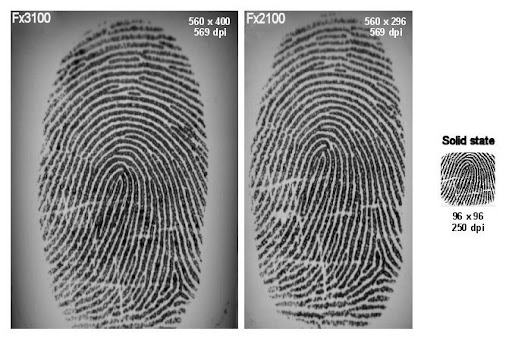
\includegraphics[width=4cm]{img/fingerprint.jpg}	
		\end{center}
		
		Объекты - образцы отпечатков пальцев

		Цель - идентифицировать человека
		
		\vspace{15pt}
		
		Особенности задачи:
		\begin{itemize}
			\item Нетривиальное преобразование входных данных в информативные признаки
			\item Требование сверхвысокой точности
		\end{itemize}			
	\end{frame}


	\begin{frame}
		\frametitle{Оценка стоимости недвижимости}
		Объекты - описание объекта недвижимости
		
		Цель - оценить стоимость
		
		Признаки:
		\begin{itemize}
			\item Бинарные: комерческая ли, наличие балкона, лифта, мусоропровода
			\item Непрерывные: площадь, год постройки дома
			\item Категориальные: район города
		\end{itemize}
		
		Особенности задачи:
		\begin{itemize}
			\item Данные могут быть очень разнородной
			\item Стоимость меняется со временем: зависимость непостоянна
			\item Влияние внешних экономических факторов
		\end{itemize}		
	\end{frame}

	
	\begin{frame}
		\frametitle{Прогнозирование объемов продаж}
		Объекты - тройка (товар, магазин, день)
		
		Цель - прогноз числа продаж
		
		\vspace{15pt}
		
		Особенности задачи:
		\begin{itemize}
			\item Разреженные данные
			\item Функция потерь сильно не симметрична
		\end{itemize}	
	\end{frame}
	
	
	\begin{frame}
		\frametitle{Ранжирование поисковой выдачи}
		Объекты - поисковой запрос
		
		Цель - формирование выдачи по убыванию релевантности
		
		\vspace{15pt}
				
		Особенности задачи:
		\begin{itemize}
			\item Очень много данных, 
			\item Требование быстрой обработки запросов
			\item Сложность формирования размеченной выборки
		\end{itemize}	
	\end{frame}
	

	\section[]{}
	
	
	\begin{frame}
		\frametitle{Резюме}
		\begin{itemize}
			\item Основные понятия: объект, признак, модель, функция потерь, метод обучения, эмпирический риск, обобщающая способность
			\item Модель - функция, заданная с точностью до параметров. Обучить модель - найти оптимальный набор параметров
			\item Проблема описывается математически $\to$ сводится к задаче оптимизации $\to$ решается
		\end{itemize}
	\end{frame}
		
\end{document}